\documentclass{article}

\usepackage{pgfplots}
\usepackage{tikz}
\usepackage{circuitikz}
\usepackage{amsmath}
\usepackage{graphicx}
\usepackage{float}
\usepackage{multirow}
\usepackage{array}
\usepackage{booktabs}
\usepackage{enumitem}
\usepackage{wrapfig}
\usepackage{pdfpages}
\usepackage{graphicx}
\usepackage{hyperref}
\usepackage{chngcntr}
\usetikzlibrary{positioning,arrows.meta,shapes.geometric}
\renewcommand{\tableautorefname}{Tabel}
\renewcommand{\sectionautorefname}{Afsnit}
\renewcommand{\subsectionautorefname}{Afsnit}
\renewcommand{\figureautorefname}{Figur}
\renewcommand{\figurename}{Figur}
\renewcommand{\contentsname}{Indholdsfortegnelse}
\renewcommand{\equationautorefname}{Ligning}
\counterwithout{figure}{section}
		\tikzstyle{startstop} = [
rectangle,
rounded corners,
minimum width=3cm,
minimum height=1cm,
text centered,
draw=black
]

\tikzstyle{process} = [
rectangle,
minimum width=3cm,
minimum height=1cm,
text centered,
draw=black
]

\tikzstyle{decision} = [
diamond,
minimum width=3cm,
minimum height=1cm,
text centered,
draw=black,
aspect=2
]

\tikzstyle{io} = [
trapezium,
trapezium left angle=70,
trapezium right angle=110,
minimum width=3cm,
minimum height=1cm,
text centered,
draw=black
]

\tikzstyle{arrow} = [
thick,
->,
>=Stealth
]
\title{Metaldetektor projekt \\Gruppe 1 \\s233986, s233988, s171678}

\begin{document}
\begin{titlepage}
	\centering
	
	{\LARGE \textbf{Metaldetektor projekt\\Gruppe 1}\par}
	\vspace{1cm}
	{\large 34621 \\ Electromagnetic sensors and digital signal processing \\ Danmarks Tekniske Universitet\par}
	\vspace{2cm}
	\begin{minipage}{0.3\textwidth}
		\centering
		\includegraphics[width=\linewidth,height=4cm,keepaspectratio,trim=1cm 1cm 1cm 1cm,clip]{Seb billede.png}\\
		\textbf{Sebastian Sørensen, s233986}
	\end{minipage}
	\hfill
	\begin{minipage}{0.3\textwidth}
		\centering
		\includegraphics[width=\linewidth,height=4cm,keepaspectratio,trim=1cm 1cm 1cm 1cm,clip]{Oli billede.jpg}\\
		\textbf{Oliver Holm, s233988}
	\end{minipage}
	\hfill
	\begin{minipage}{0.3\textwidth}
		\centering
		\includegraphics[width=\linewidth,height=4cm,keepaspectratio,trim=1cm 1cm 1cm 1cm,clip]{Bilal billede.png}\\
		\textbf{Bilal Alali, \newline s171678}
	\end{minipage}
	
	\vfill
	{\large \today}
	
\end{titlepage}
	\newpage
	\tableofcontents
	\newpage
\section{Introduktion}
	\begin{figure}[H]
		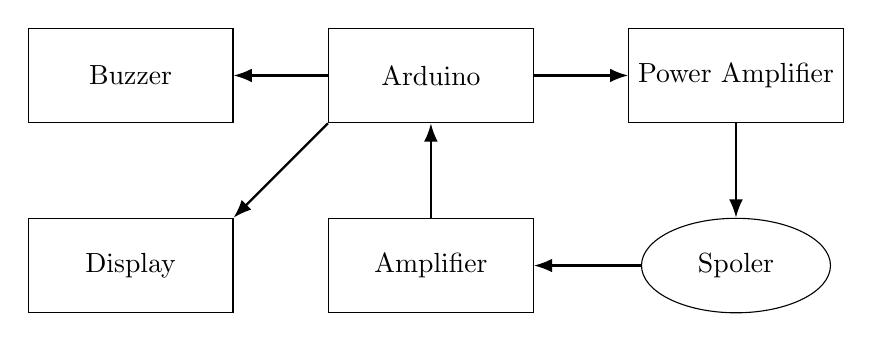
\begin{tikzpicture}[
			block/.style={
				draw,
				rectangle,
				minimum width=2.6cm,
				minimum height=1.2cm,
				align=center
			},
			io/.style={
				draw,
				ellipse,
				minimum width=2.4cm,
				minimum height=1.2cm,
				align=center
			},
			arrow/.style={
				->,
				thick,
				>=Latex
			}
			]
			
			% Nodes
			\node[block] (arduino) {Arduino};
			\node[block, left=1.2cm of arduino] (buzzer) {Buzzer};
			\node[block,below=1.2cm of buzzer] (display) {Display};
			\node[block, right=1.2cm of arduino] (pa) {Power Amplifier};
			\node[block, below=1.2cm of arduino] (amp) {Amplifier};
			\node[io,below=1.2cm of pa] (coils) {Spoler};
			
			% Arrows
			\draw[arrow] (arduino) -- (pa);
			\draw[arrow] (pa) -- (coils);
			\draw[arrow] (coils) -- (amp.east);
			\draw[arrow] (amp.north) -- (arduino.south);
			\draw[arrow] (arduino.south west) -- (display.north east);
			\draw[arrow] (arduino.west) -- (buzzer.east);
			
		\end{tikzpicture}
		\caption{Overordnet moduldiagram af systemet}
		\label{fig:ModuleDiagram}
	\end{figure}
\section{Analyse}
\section{Design}
	\subsection{Analogt design}
		\subsubsection{Energiberegninger}
			Vi undersøgte os frem til at batteriet har en kapacitet på $550$mAh. Da batteriet aflades fra 9V til 6V, har vi lavet udregningen:
				$$E_{tot}=V\cdot I\cdot3600 \iff E_{tot}=\frac{9V+6V}{2}\cdot0.55\text{A}\cdot3600\text{s}=14850\text{J}$$
			Ved måling af strømforbruget finder vi at OLED-display og Arduinoen forbuger $\approx76.2\text{mA}$. Dette giver os $$E_{MCU}=5\text{V}\cdot76.2\cdot10^{-3}\text{A}\cdot3600\text{s}=1371.6\text{J}$$Vi reserverer $15\%$ af batteriet som buffer, for at være sikker på at overholde kravene. Resten af energien kan bruges til TX-spolen.
			$$E_{TX}=E_{tot}\cdot(1-0.15)-E_{MCU}=11250.9J$$
		\subsubsection{Spoleberegninger}
			\begin{center}
				\textbf{TX-spole}
			\end{center}
			Ved resonans kan spændingen gennem spolen approksimeres ved grundtonen i fourierrækken  $$a_n\approx2\left(\frac{A}{n\pi}\right)\sin\left(\frac{n\pi}{2}\right)=2\left(\frac{9\text{V}}{\pi}\right)\sin\left(\frac{\pi}{2}\right)=5.73\text{V}$$
			Hvorved RMS-spændingen kan bestemmes $$V_{RMS}=\frac{a_n}{\sqrt{2}}=4.05\text{V}$$
			Derved kan vi nu beregne strømmen vi kan sende igennem spolen
			$$I_{TX}=\frac{E_{TX}}{t\cdot V_{RMS}}=\frac{11250.9\text{J}}{3600\text{s}\cdot4.05\text{V}}=0.4628\text{A}$$
			Radiussen på TX-spolen vælges til $r_{TX}=10cm$, med $D_{TX}=\text{Ø}0.4\text{mm}$. Derved kan antallet af viklinger beregnes ved
			$$R_{TX}=\frac{V_{RMS}}{I_{TX}}=8.754\Omega$$
			$$N_{TX}=\frac{R_{TX}\cdot\left(\frac{D_{TX}}{2}\right)^2} {2\cdot r_{TX}\cdot\rho_{cu}}=\frac{8.754\Omega\cdot\left(\frac{0.4\text{mm}}{2}\right)^2}{2\cdot10\text{cm}\cdot1.77\cdot10^{-8}\Omega\cdot m}=98.9$$ hvilket afrundes til $N_{TX}=99$.\newline
			Selvinduktansen i spolen findes ved
			$$L=\frac{0.394\cdot r^2\cdot N^2} {9\cdot r+10A}=\frac{0.394\cdot10^2\cdot99^2} {9\cdot10+10}=3.855\text{mH}$$
			For at kunne lave Arduino'ens firkantsignal til en sinuskurve anvendes et resonanskredsløb, som har resonansfrekvens på $2\text{kHz}$. Størrelsen af kondensatoren findes ved at løse ligningen
			\begin{equation}
			\label{eq:Cresonance}
			 f=\frac{1}{2\pi\sqrt{LC}} \iff 2\text{kHz}=\frac{1}{2\pi\sqrt{3.855\text{mH}\cdot C}} \implies C=1.642\mu\text{F}
			 \end{equation}
			Magnetfeltet fra TX-spolen beregnes, da bucking-spolen skal udligne B-feltet fra TX-spolen, for på den måde at tilsikre at vi kun måler på magnetfeltet fra metallet i detektoren. 
			$$|B|=\frac{\mu_0I_{TX} N_{TX}}{2r_{TX}}=\frac{4\pi\cdot10^{-7}\frac{\text{H}}{\text{m}}\cdot0.4628\text{A}\cdot99}{2\cdot10\text{cm}}=287.6\mu\text{T}$$
			\begin{center}
				\textbf{Bucking-spole}
			\end{center}
			Derved kan Bucking-spolen beregnes. Vi vælger en radius på $r_{Buck}=5\text{cm}$, og antallet af viklinger beregnes ved
			$$|B|=\frac{\mu_0\cdot I_{TX}\cdot N_{Buck}}{2\cdot r_{Buck}} \iff 287.6\mu\text{T}=\frac{4\pi\cdot10^{-7}\cdot0.4628\text{A}\cdot N_{Buck}} {2\cdot5\text{cm}}\implies N_{Buck}=49.458$$ hvilket afrundes til $N_{Buck}=50$.
			\begin{center}
				\textbf{RX-spole}
			\end{center}
			For at opnå en god følsomhed på sensoren, er vi opmærksomme på at induktansen i RX-spolen skal være minimum $L_{RX}=10\text{mH}$. Derved beregnes antallet af viklinger ved
			$$10\cdot10^3=\frac{0.394\cdot r_{RX}^2\cdot N_{RX}^2} {9r_{RX}+10A_{RX}}=\frac{0.394\cdot5^2\cdot N_{RX}^2} {9\cdot5+10}\implies N_{RX}=236$$
			\subsubsection{Power Amplifier}
			\begin{figure}[H]
				\centering
				\begin{circuitikz}[american,scale=0.8]
					% Q5
					\draw (3,3) node[npn,anchor=B,label={[align=left]right:{$Q_1$\\BC337-25}}] (Q5){};
					% Q6
					\draw (6,4) node[pnp,anchor=B,label={[align=left]right:{$Q_3$\\BC327-40}}](Q6){};
					% Q3
					\draw (6,7) node[npn,anchor=B,label={[align=left]right:{$Q_2$\\BC337-25}}](Q3){};
					% Q7
					\draw (8,3) node[npn,anchor=B,label={[align=left]right:{$Q_5$\\BC337-25}}] (Q7){};
					% Q4
					\draw (8,8) node[pnp,anchor=B,label={[align=left]right:{$Q_4$\\BC327-40}}] (Q4){};
					\draw	(0,0) node[ground]{} to [short,-*]++(0,0) 
					to[sV, l={\shortstack{2\,kHz\\0--5\,V}}] (0,3)
					to [R={\shortstack{$10\text{k}\Omega$\\$R_3$}}] ++(2,0)
					to [R={\shortstack{$10\text{k}\Omega$\\$R_2$}}] ++(0,-3) to [short,-*]++(0,0);
					\draw (Q5.B) to [short,-*] (2,3);
					\draw (Q5.E) to [short,-*] ++(0,-2);
					\draw (Q5.C) to [short,-*] ++(0,1.5)
					to [short,-*] ++(1.95,0) -- (Q3.B) -- (Q6.B);
					\draw (Q5.C) -- ++(0,4) to [R={\shortstack{$10\text{k}\Omega$\\$R_1$}}] ++(0,2.25) to [short,-*]++(0,0);
					\draw (Q3.C) to [short,-*] ++(0,0)  to [R={\shortstack{$10\text{k}\Omega$\\$R_5$}}] ++(0,2.25) to 		[short,-*]++(0,0);
					\draw (Q4.E) to [short,-*]++(0,1.25);
					\draw (Q3.E) to [short,-*] ++(0,-0.8) to [short,-*]++(2,0);
					\draw (Q6.E) --++(0,1);
					\draw (Q7.C) to (Q4.C);
					\draw (Q6.C) to [short,-*]++(0,-0.05) to (Q7.B);
					\draw (Q6.C) --++(0,0) to [R={\shortstack{$10\text{k}\Omega$\\$R_6$}}]++(0,-3) to [short,-*]++(0,0);
					\draw (Q4.B) --++(-1,0);
					\draw (Q7.E) to [short,-*]++(0,-2);
					\draw (11,0) to[D,l={\shortstack{$D_1$\\1N4148}}](11,3) to ++(0,2.25) 	coordinate(S1);
					\draw (S1) to [short,-*]++(0,0);
					\draw (S1) --++(-2.2,0);
					\draw (S1)  to [D,l={\shortstack{$D_2$\\1N4148}}]++(0,2) --++(0,3) to ++(-10,0) 	to 		[vsource=$9\text{V}$]++(0,-2) coordinate(9V-);
					\draw (S1) to [C={\shortstack{$1642\text{nF}$\\$C_1$}}] ++(3,0) to [L={\shortstack{$3.855\text{mH}$\\$L_1$}}]++(0,-2) 	to 		[R={\shortstack{$8.75\Omega$\\$R_7$}}]++(0,-1.75) to ++(0,-1.5) to ++(-14,0);
					\draw (11,0) to [short,-*]++(0,0);
					\node[ground] at (9V-){};
				\end{circuitikz}
				\caption{Power amplifier kredsløb til at øge strømmen gennem TX-spolen.}
				\label{fig:PA}
			\end{figure}
			Ovenfor ses vores design af effektforstærkeren, som bruges til at forstærke signalet fra Arduino'en til at kunne drive TX-spolen. Kredsløbet virker ved:
			\begin{itemize}
				\item Firkantsignalet sendes ind i forstærkeren gennem en modstand som beskytter Arduino'en og styrer strømmen ind i transistoren $Q_1$. 
				\item Transistor-konfigurationen fungerer som en forstærker som via. en styrestrøm kontrollerer en større strøm fra batteriforsyningen (9V batteriet), som driver TX-spolen.
				\item TX-spolen ($L_1$) genererer et magnetfelt ved resonansfrekvensen
				\item Kondensatoren ($C_1$) er beregnet (\autoref{eq:Cresonance}) således at der opstår resonans ved detektionsfrekvensen på $2\text{kHz}$
				\item Modstanden $R_7$ repræsenterer den ohmske modstand i TX-spolen.
				\item Dioderne $D_1$ og $D_2$ beskytter kredsløbet fra den induserede spænding i spolen.
			\end{itemize}
		\subsubsection{Filtrering af spolesignal}
			\begin{figure}[H]
				\centering
				\begin{circuitikz}[american]
					\draw (0,0) node[ground]{} to [sV,l=$V_{RX coil}$] ++ (0,2) to [L=$11.75\text{mH}$] 	++(2,0) to [R=$41.9\Omega$]++(2,0)
					coordinate(N1) to [short,-*]++(0,0) to [C=$80\text{nF}$]++(0,-2) to 	[short,-*]++(0,0);
					\draw (N1) --++(2,0) coordinate (Vout) to [generic={\shortstack{$50\text{k}\Omega$\\$Z_1$}}]++(0,-2) to 	[short,-*]++(0,0)coordinate(VR) to (0,0);
					\draw (Vout) to [short,-*]++(0,0) --++(2,0) to node[ocirc]{}++(0,0) 	coordinate(V+);
					\draw (VR) --++(2,0) to node[ocirc]{}++(0,0) coordinate(V-);
					\draw (V+) to [open,v=$V_{filtered}$] (V-);
				\end{circuitikz}
				\caption{Kredsløb til at filtrere støj væk ($\approx\frac{Fs}{2}=4\text{kHz}$) inden signalet bliver forstærket (som vist i \autoref{fig:OPAMP}). Modstanden på $50\text{k}\Omega$ repræsenterer indgangsimpedansen i operationsforstærkerkredsløbet.}
				\label{fig:RXfilter}
			\end{figure}
			Som det ses i figuren, er $V_{filtered}=V_{Z_1}$. Filterets overføringsfunktion kan opstilles ved almindelig spændingsdeling, dvs. $$H(\omega)=\frac{R_2\cdot\frac{1}{j\omega C}} {R_1+Z_1+R_2\cdot\frac{1}{j\omega C}}$$ hvorefter fasen kan analyseres ved $$\phi(\omega)=\tan^{-1}\left(\frac{\Im\{H\}}{\Re\{H\}}\right)$$
			og amplitude responset ved $$H_{dB}=20\log10(H)$$
			\newline
			Ifølge Shannon's sampling teorem ved vi at $F_{max}<\frac{F_s}{2}$. Da vi ikke har noget signal som ligger over $\frac{F_s}{2}=4\text{kHz}$ anvender vi dette filter, for at undgå problemer med aliaseringer. Filteret er designet således at fasen bliver påvirket mindst muligt, da det netop er fasen vi bruger til at skelne mellem materialer.
				\begin{figure}[H]
					\caption{RX-filterets fase- og magnitude respons, med markering af 4.2kHz}
					\label{fig:dft-plot1}
					\includegraphics[width=\textwidth]{"DFT plot1"}
				\end{figure}
			Da metaldetektorens følsomhed overfor frekvenser afhænger af bl.a temperatur, har vi valgt at designe filteret efter et udgangspunkt på $4.2\text{kHz}$. Som det ses i plottet får vi dæmpet det værste af eventuelt højfrekvent støj, samtidigt med at vi aflæser fasen nogenlunde præcist med udgangspunkt i $4.2\text{kHz}$. 
			
			\subsubsection{Forstærkning af spolesignalet}
				\begin{figure}[H]
					\centering
					\begin{circuitikz}[american]
						\draw (0,-2) node[ground]{} to [short,-*]++(0,0) to 		[vsourcesin,l=$V_{filtered}$]++(0,2)
						to [C=$1\mu\text{F}$]++(2,0) to [short,-*]++(0,0) coordinate(N1);
						\draw (N1) to [R=$100\text{k}\Omega$]++(0,-2) to [short,-*]++(0,0);
						\draw (N1) to [R=$100\text{k}\Omega$]++(0,4) to [short,-*]++(0,0) 	coordinate(N2) 	to [vsource,l=$5\text{V}$]++(0,2) --++(-2,0) coordinate(V-);%--++(0,-8) --++(10.8,0) coordinate(N5); % Linje til ground her
						\node[ground] at (V-){};
						\draw (0,-2) to ++(9,0) to node[ocirc]{}++(0,0) coordinate(Vout-);
						\draw (6,3.5) node[op amp,yscale=-1,label=south:MC6002] (opamp){};
						\draw (opamp.+) to (N2);
						\draw (opamp.-) to [short,-*]++(0,-1) coordinate(N3) to 		[R=$1\text{k}\Omega$]++(0,-2) to [C=$1\mu\text{F}$]++(0,-2) to [short,-*]++(0,0);
						\draw (N3) to [potentiometer,l_=$0-200\text{k}\Omega$] ++(3,0) to [short,-*]++(0,1.5) 		coordinate(Vo);
						\draw (Vo) to (opamp.out);
						\draw (Vo) --++(1.25,0) to node[ocirc]{}++(0,0) coordinate(Vout+);
						\draw (Vout+) to [open,v=$V_{out}$](Vout-);
						%	\draw (Vo) --++(1,0) to [open,v^=$V_{out}$](N5);
					\end{circuitikz}
					\caption{Kredsløb til at forstærke den filtrerede spænding fra RX-spolen op, inden det læses ind i MCU ADC'en.}
					\label{fig:OPAMP}
				\end{figure}
	\subsection{Digitalt design}
		\subsubsection{Moduldiagram og introduktion}
			\begin{figure}[H]
				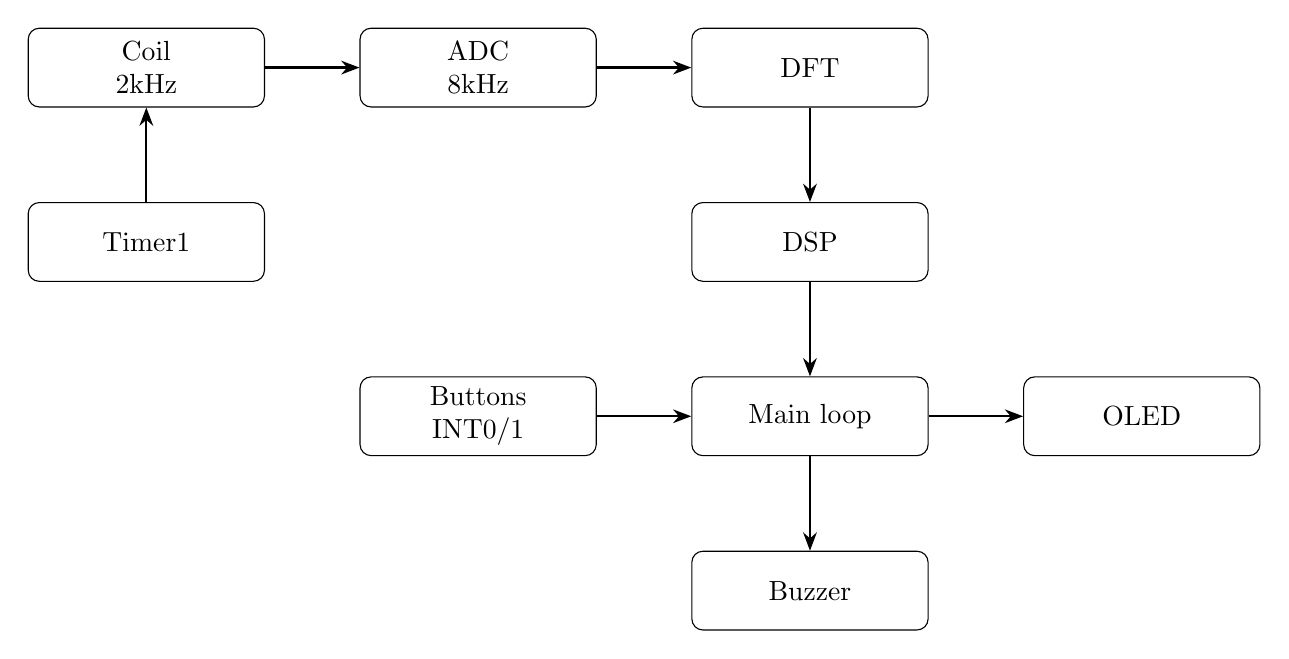
\begin{tikzpicture}
					%Nodes
					\node[startstop,align=center] (coil) {Coil\\2kHz};
					\node[startstop,align=center,right=1.2cm of coil] (adc) {ADC\\8kHz};
					\node[startstop,right=1.2cm of adc] (dft) {DFT};
					\node[startstop,below=1.2cm of dft] (dsp) {DSP};
					\node[startstop,below=1.2cm of coil] (timer1) {Timer1};
					\node[startstop,below=1.2cm of dsp] (main) {Main loop};
					\node[startstop,right=1.2cm of main] (oled) {OLED};
					\node[startstop,align=center,left=1.2cm of main] (buttons) {Buttons\\INT0/1};
					\node[startstop,below=1.2cm of main] (buzzer) {Buzzer};
					%Arrows
					\draw[arrow] (coil.east) -- (adc.west);
					\draw[arrow] (adc.east) -- (dft.west);
					\draw[arrow] (dft.south) -- (dsp.north);
					\draw[arrow] (timer1.north) -- (coil.south);
					\draw[arrow] (dsp.south) -- (main.north);
					\draw[arrow] (buttons.east) -- (main.west);
					\draw[arrow] (main.east) -- (oled.west);
					\draw[arrow] (main.south) -- (buzzer.north);
				\end{tikzpicture}
				\caption{Overordnet moduldiagram af systemet}
				\label{fig:DigitalModulDiagram}
			\end{figure}
		\subsubsection{Brugerinteraktion}
		\subsubsection{DFT algoritme og sampling}
		\begin{figure}[H]
			\centering
			\includegraphics[width=0.5\linewidth]{"DFT plot"}
			\caption{Grafisk illustration over princippet bag DFT-algoritmen. Ved at vælge $F_d=\frac{F_s}{4}$, undgår vi at lave komplicerede komplekse beregninger.}
			\label{fig:dft-plot}
		\end{figure}
		\subsubsection{Tilstandsmaskine}
		\subsubsection{Digital signal behandling}

\section{Implementering og test}


\section{Ansvarsområder (hvem har lavet hvad)}
\begin{center}
	\textbf{Fælles}
\end{center}
\begin{itemize}
	\item Vikling af spoler
	\item Implementering af kredsløb
\end{itemize}

\begin{center}
	\textbf{Bilal}
\end{center}
\begin{itemize}
	\item 3D-print
	\item Power Amplifier
	\item Spoleberegninger
	\item Energiberegninger
\end{itemize}
\begin{center}
	\textbf{Sebastian}
\end{center}
\begin{itemize}
	\item C-programmering
	\item RX-filter
	\item Grafik til rapport (plots, kredsløbstegninger,indskrivning af rapport)
	\item 
\end{itemize}
\begin{center}
	\textbf{Oliver}
\end{center}
\begin{itemize}
	\item C-programmering
	\item 
\end{itemize}


\section{Konklusion}

	
\section{Appendix}
	\subsection{Gantt kort}
	\subsection{Mødereferater}
\end{document}